\documentclass[twoside,11pt]{cergdoc}
\usepackage{graphicx}
\usepackage{amsmath}
\usepackage{listings}

\newcommand\thead[1]{\multicolumn{1}{c}{\textbf{#1}}}
\newcommand\theadr[1]{\multicolumn{1}{c|}{\textbf{#1}}}
\newcommand{\ITwoC}{I\textsuperscript{2}C }

\begin{document}

\lstset{%
  basicstyle=\ttfamily,
  language=C,
  otherkeywords={bis.b,bis.w,bic.b,bic.w,bit.b,bit.w,mov.b,mov.w,dec.b,dec.w,jnz,jmp},
  commentstyle=\color{cerglightblue},
  keywordstyle=\color{cergpink},
  numberstyle=\color{cergpred},
  stringstyle=\color{cergblue},
  identifierstyle=\color{cergpurple}
}

\title{eXtended eXternal Benchmarking eXtension -- XXBX}
\subtitle{XXBX Getting Started v1.0}
\author{Matthew R. Carter \and Raghurama R. Velegala \and John Pham \and Jens-Peter Kaps}
\email{jkaps@gmu.edu}
\affiliation{George Mason University\\
  Fairfax, Virginia}
\topicpic{xxbx-slide}

\maketitle

\tableofcontents

% -----------------------------------------------------------------------------
\chapter{Introduction}
% -----------------------------------------------------------------------------
  \section{Benchmarking}
  \section{Metrics}
For embedded software cryptography implementations, the areas of interest are
ROM usage, Random Access Memory (RAM) usage, throughput, and power. This:
differs from non-embedded environments, where typically only throughput is
considered when evaluating performance, as disk storage (analogous to ROM), RAM,
and power are plentiful.  

    \subsection{Throughput}
Throughput for cryptographic software is given in cycles per byte, in an effort
to be independent of different clock speeds within the same family of CPU, as
well as variable clock speeds due to power saving \cite{sha3bench}. This only
helps with variations in clock speeds, or comparing between otherwise identical
architectures with varying features such as a Single Instruction Multiple Data
(SIMD) unit like NEON or SSE. Results from different
instructions per clock and/or instruction formats still cannot be compared with
each other.

    \subsection{ROM}
ROM usage is typically determined by the program code as well as any constants,
and preinitialized variable data. Microcontrollers have anywhere between
a few kibibytes to a mebibyte of ROM. This is typically consists of the 
\texttt{.text} (code and constants) and \texttt{.data} (initialization data for
static buffers in RAM) sections in a compiled binary.

    \subsection{RAM}
RAM is organized into statically allocated RAM set aside at the beginning of
program execution, stack memory that grows as function call chains get deeper,
and dynamic allocations via \texttt{malloc} and similar functions. The statically
allocated RAM is divided into \texttt{.bss} and \texttt{.data} sections.
\texttt{.data} is for preinitialied modifiable buffers in RAM that also take up
space in ROM for the initialization data as previously mentioned, while
\texttt{.bss} is for uninitialized buffers that only occupy RAM.

    \subsection{Power}
As software ultimately runs on hardware containing a processor, the same
constraints on power that affect hardware affects software. The power and energy
used is influenced by which processing units the software uses, the
microprocessor the software runs on, the clock speed and the total running time.

% -----------------------------------------------------------------------------
\chapter{Previous Work}
% -----------------------------------------------------------------------------
There are many existing tools for benchmarking cryptographic software.
The System for Unified Performance Evaluation Related to Cryptographic Operations and Primitives
(SUPERCOP) is a cryptographic benchmarking tool that benchmarks a large variety
of cryptographic primitives on general purpose computers\cite{supercop}.
However, it is not capable of being run on embedded platforms, and lacks
important metrics for embedded such as ROM and RAM usage.

Two software benchmarking tools for embedded are XBX\cite{xbx} and
FELICS \cite{felics}\cite{dinu_triathlon}. XBX is an tool for evaluating
hash functions packaged for SUPERCOP, and primarily runs implementations on
actual hardware. 

FELICS is a newer tool, focused on lightweight primitives, and current
lightweight block ciphers, and adds cycle-accurate simulation for a variety of
platforms as well as running implementations on actual hardware. 

In this paper, we further extend XBX to cover AEAD primitives in addition to
XBX, and allow easy extensibility to support the rest of the operations SUPERCOP
supports. In addition, we intend to add the ability to measure power and energy
consumption.

  \section{SUPERCOP}
SUPERCOP ``[...] is a toolkit developed by the VAMPIRE lab for measuring
the performance of cryptographic software \cite{supercop}.'' The project collects
and benchmarks many implementations across many primitives on multiple
platforms. It consists of a series of shell scripts and test harnesses that
compile implementations and their dependencies across different compilers and
flags. It then verifies outputs and correctness, and measures performance
characteristics. Power measurements, code size, and memory usage data
measurements are not supported.

  \section{XBX}
The eXternal Benchmarking eXtension (XBX)\cite{xbx} is an extension to SUPERCOP that covers
platforms that are not capable of hosting a compiler and require cross-compilation,
such as microcontrollers or small embedded Linux systems. It reuses the
primitive implementations collected by the SUPERCOP project (which it refers to as
an ``algopack''), as well as others, and
attempts to retain the same output data format. XBX is able to test multiple
implementations across multiple primitives  with multiple compilers and compiler
flags without intervention, which is important with the large number of
combinations to be tested. Due to the importance of small code and memory size for
embedded platforms, these are also measured and recorded.

% -----------------------------------------------------------------------------
\chapter{XXBX System}
% -----------------------------------------------------------------------------
  \section{Overview}
The XXBX system is comprised of four main
components:

\begin{figure}[ht]
  \begin{center}
    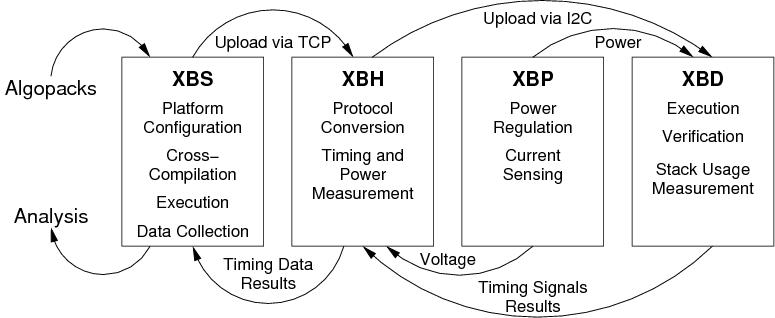
\includegraphics[scale=0.8]{figures/xxbx_block}
    \caption{Block Diagram of the XXBX System}\label{fig:xxbxsystem}
  \end{center}
\end{figure}



The communication between the XBS and XBH uses
TCP/IP over Ethernet, while I2C is used between
XBH and XBD. A buffer is used to queue the
commands received from the XBS before sending
them to XBD.

  \section{XXBX Software -- XBS}
The XBS is software running on a PC that consists of scripts that handle
compilation of algopacks and firmware upload to the
XBH, as well as data aggregation and logging. Static allocation of RAM and ROM
usage is also calculated from the compiler output. Multiple compilers and
compiler flags are used to compile an implementation.

  \section{XXBX Harness -- XBH}
The XBH is a board that translates high level commands from the XBS sent via
TCP/UDP to series of commands over a protocol understood by the XBD
(\ITwoC, RS232, or Ethernet). Future references to the XBS communicating to the
XBD refers to this.
It also measures execution time via the timer capture pins, which precisely
record the time that an edge event occurs. Because not all XBD
platforms support cycle counters, the execution time is measured externally.

  \section{XXBX Power Shim -- XBP}
 The power is measured
using a shunt resistor circuit. The current is amplified
here so that ADC on the XBH can measure it.


  \section{XXBX Device Under Test -- XBD}
The XBD is the platform hardware that the primitive implementations are tested
on. It performs the execution task and
notifies the XBH of start and completion via a general-purpose input/output
(GPIO) pin connected a timer capture pin on the XBH. It also returns the maximum
stack RAM used to the XBH over the XBD$\leftrightarrow$XBH communication
    channel. The supported platforms are ARM, AVR, MSP430, and MIPS. 

The XBD code consists of two components. One is a small bootloader that is
flashed once to XBD that performs basic calibration and self programming of the
primitive implementations over the communications channel. 

The second component is a test harness that is linked with the
primitive implementation that is downloaded over the communication channel. This
code is responsible for signaling start and stop, supplying the implementation
with input data, verifying the correctness of the algorithm implementation and
returning the output to the XBH. 

Both of these are linked to code which provides device specific drivers for
communication and execution signaling, as well as stack measurement. 


% -----------------------------------------------------------------------------
\chapter{First Steps}
% -----------------------------------------------------------------------------
  \section{Requirements}
  \section{Installation}

    \subsection{XBH}
The XBS connects to the XBH via Ethernet. The TCP/IP parameters can be set
in the file \verb|xbx/xbh/xbh_config.h|. All IP addresses are to be specified
in hexadecimal. An example is shown below.

\begin{cergbox}{XBH TCP/IP Configuration}
\begin{lstlisting}
#define XBH_HOSTNAME    "xbh"
#define TCP_XBH_PORT    22595
#define XBH_IP4_STATIC  1          // no dhcp, use static address
#define XBH_IP4_ADDR    0xC0A80A10 // 192.168.10.16   
                     // C0-192, A8-168, 0A-10, 10-16
#define XBH_IP4_NETMASK 0xFFFFFF00 // 255.255.255.0
\end{lstlisting}
\end{cergbox}

The XBS will try to connect to the XBH by name "xbh". Hence, the name "xbh" has to 
be mapped to the correct IP address. You can edit your \verb|\etc\hosts| file
and add the following line.

\begin{center}
\verb|192.168.10.16    xbh|
\end{center}

After you have made settings appropriate to your network, you have to compile
the XBH code. This requires that a GCC ARM compiler is installed on your system.
One option is to install \emph{Code Composer Studio (CCS)} from \emph{Texas Instruments}
which can be found at \url{http://www.ti.com/tool/CCSTUDIO}. After installation
start CCS as \textbf{root} to install all updates and make sure that 
\emph{ARM GCC} is selected in the \emph{App Center} of CCS. Then add the location
of the ARM GCC to your \emph{PATH} environment variable of your shell. The text 
\texttt{VERSION} in the example below has to be replaced with the version installed
on your system. 
The ARM GCC executable is typically called \texttt{arm-none-eabi-gcc}.

\begin{center}
\lstinline|export PATH=/opt/ti/ccsv8/tools/compiler/gcc-arm-none-eabi-VERSION/bin/:$PATH| 
\end{center}

Now enter the \verb|xbx/xbh| directory and build the XBH executable by typing 

\begin{lstlisting}
make
\end{lstlisting}

In oder to program the XBH, first install \emph{openocd} from your Linux distribution.
Then configure \emph{udev} for the XBH by creating a new file called
\texttt{99-tiva-launchpad.rules} in \verb|/etc/udev/rules.d/|.

\begin{cergbox}{Contents of \texttt{/etc/udev/rules.d/99-tiva-launchpad.rules}}
\small\begin{lstlisting}
SUBSYSTEM=="tty", ATTRS{idVendor}=="1cbe", ATTRS{idProduct}=="00fd", 
GROUP="dialout", MODE="0666"
\end{lstlisting}
This text should be in one line.
\end{cergbox}

In order to activate this rule you can either restart your computer or issue the
following commands on the command line.

\begin{lstlisting}
systemctl restart udev 
udevadm trigger
udevadm settle
udevadm control -R
\end{lstlisting}

Now the system is ready to program the XBH. Connect the XBH with a USB cable plugged into
the USB port labled \emph{DEBUG} on the XBH. Start the debugger \verb|arm-tiva_c-eabi-gdb|
and issue the following commands in the debugger shell.

\begin{lstlisting}
source .gdbinit
load
c
\end{lstlisting}

Start a terminal program (for example \emph{minicom} 
and point it to your XBH. The XBH typically uses \verb|/dev/ttyACM0|.
You can verify this with the output of the \texttt{dmesg} command. Connect the XBH to the
Ethernet and press the \emph{Reset} button on the XBH. It should print its main 
settings into the terminal. Now your XBH is ready.

\subsection{XBD}
Example ek-tm4c123gxl

same C-compiler as used for XBH
go to 
\verb|xbx/xbs_xbd/platforms/ek-tm4c123gxl_16mhz/bootloader/makefiles|
type make

make sure only the XBD is connected to your computer and the xbh is not.

start
arm-none-eabi-gdb

\begin{lstlisting}
source .gdbinit
load
c
\end{lstlisting}

done

  \section{Example Run}
Prior to running any scripts, the XBD is initialized by compiling the
platform-specific bootloader and flashing it normally (i.e. using a programming
cable). 
This bootloader has the responsibility of downloading code from the XBH. This allows board-specific
programming tools to be avoided, besides the initial setup, and thus all
subsequent operations can be performed by the XBS over a network, potentially as
part of a farm.

Scripts from the XBS compile all implementations of primitives, linking with
the hardware abstraction layer (HAL) and the test harness, with the possible
\{compiler, flags\} defined in the platform support files. The number of generated
application binaries should be $\{\rm{compilers,flags}\}\times\rm{primitive
implementations}$. The UNIX \texttt{size} command is run on the generated
application binaries to get the sizes of
\texttt{.bss}, \texttt{.data}, and \texttt{.text}. Implementations listed in a
platform-specific blacklist and a global blacklist are omitted from compilation.
Binaries are compiled into Executable and Linkable Format (ELF) which is then
converted into Intel Hex (IHEX) for transfer to the XBH. XBX checks to see if
a binary will fit, otherwise it will not be loaded later.

The XBS then orders the XBH to calibrate cycle calculations on the XBD. The
XBD's bootloader executes a busy loop for a fixed number of cycles determined by
the HAL. The XBH measures the physical time executed. The cycles run is then
calculated by dividing the measured time by the clock rate.

The XBS then sends the application binary to the XBD. This is sent one flash
block at a time, as existing data on the flash must be erased, and this can only
be done one block at a time. After each block is completely received, the XBD
writes the block from the RAM buffer to flash
memory. 

When all blocks are received, the XBD will switch to the application by
calling the address of the application's entry point, which is set to a fixed
address by linker scripts or compiler flags. This is the code
that copies \texttt{.data} from ROM to RAM, zeroes out \texttt{.bss}, and
initializes the stack pointer, then calls main. This is typically defined by the
C runtime, and is often known as ``crt0''. However the ARM Stellaris platform has
this defined as part of the HAL, as it is based off example code provided by the
chip vendor which also does this. As the initialization is run, the previous
call stack and static memory allocations of the bootloader is obliterated and
replaced with that of the application. A similar procedure is applied to switch
back to the bootloader after application execution. 

Once in application mode, the XBD is ordered to verify correct execution of the
primitive implementation. This is done by hashing repeatedly (XBX only supports hashing), mixing
in the results of the previous hash, and comparing the results to that generated
by the reference implementation on a PC. 

The XBD is then ordered to perform the actual benchmarks. Data randomly
generated by the XBS of varying lengths (0, 1, 2, 4, 8, 16, 32, 64, 128, 256, 512, 576, 1024,
1536, and 2048 bytes) is sent to the XBD, and hashed. The XBD signals to the XBH
the start and stop times by setting a signal line low upon start and raising it
high again upon stop. Any delays in detecting timing should be symmetrical
across start and stop and should not affect the result \cite{xbx}. This is
repeated multiple times (defaulting to 5). 

Stack usage is measured by painting memory with a canary value from the top of
the statically allocated memory sections to the current location of the stack
before executing the implementation. After execution, the number of addresses
still containing the canary value and not overwritten by the call stack growing
when the implementation returns is subtracted from the number of addresses
painted to determine the amount of stack memory used. 

% insert picture of stack painting


Upon execution completion, the XBS will request the measured stack value from
the XBD and the timing results from the XBH. These values are logged and the
process repeats starting with loading the next application binary, until all of
them are tested. 

Results are output


%------- merge text above (XBX) with text below (XXBX) -------

First, the configuration in \texttt{config.ini} is edited. This specifies
whitelists and blacklists of implementations, the target operation, the target
platform, paths, parameters, dependencies, etc. We assume that resuming a failed
run will not involve changing the target operation and platform. Logging levels
can be configured in \texttt{logging.ini}, and uses Python's built-in logging
framework. 

Then \texttt{compile.py} is then run. This creates the file \texttt{data.db},
used to store results, configuration, and other detailed
information. \texttt{config.ini}, a platform-specific config file, and various
blacklist files are all parsed. 

If a whitelist exists in \texttt{config.ini}, only the
implementations in this list will be built (and later run), otherwise all
implementations available in the specified operation and primitives are built,
excluding those specified in the blacklist. There is a blacklist in config.ini,
specific to the run, as well as a global blacklist for implementations that are
broken, and platform specific blacklists for implementations that are broken on
specific platforms. Hashes of all implementation and platform code are taken to
ensure exact replication of results, if required.

Once the configuration is assembled, the compile script generates the makefiles
and header files for each implementation and builds the code for the XBD for
each implementation $\times$ \{compiler, flag\}. This proceeds quickly, as the
script spawns as many subprocesses as there are cores to execute builds. We
decided to run multiple makefiles simultaneously as opposed to running GNU make
with the \texttt{-j} flag, which does parallelization at the makefile level, as
even with \texttt{-j}, the makefiles would stall trying to build something that
would not build, e.g. attempting to compile x86 assembly to ARM. Running
separate makefiles in parallel builds more quickly, by allowing stalls to not
block other tasks. The \texttt{size} command is run as in original XBX on the
compiled binaries, and the values saved in the database. We decided to limit the
maximum static memory allocations to 3/4ths the total available RAM, leaving the
remainder for stack growth, for both the Tiva-C and the MSP430 XBDs in the
platform configuration.

As the builds use GNU \texttt{make}, rebuilds do not require recompiling everything from
scratch, only the code that changed or that was interrupted. Original XBX did
not use makefiles. It copied all source files to a build directory, and compiled
the source files together all at once, which meant all files are always rebuilt
even if nothing changed. 

Unlike XBX, and like SUPERCOP, primitive implementations can depend on other
implementations. However, the relations have to be explicitly defined, as there
are multiple metrics for what a good implementation is, unlike SUPERCOP.

Once a build succeeds, the \texttt{execute.py} script is run. The configuration
used from the last build is loaded from \texttt{data.db}, if \texttt{config.ini}
has not changed between the last build and calling \texttt{execute.py}. Behavior
is undefined if \texttt{config.ini} or blacklists or code are modified between
calls of \texttt{compile.py} and \texttt{execute.py}. Calibration is run as in
original XBX.

%TODO Explain verification for AEAD and Hash

For each successfully compiled implementation, the binary is loaded into the XBD
and tests are run, as mentioned in section \ref{sec:prim_test}. These tests can
be run multiple times if configured for such, however they take a considerable
amount of time. Afterwards, the XBS generates data to send to the XBD for
performance testing, as specified in the config file. A python object defining
the parameters, how to generate them, and how to handle what is returned by the
XBD is required to support an operation, and as previously mentioned, we have
hash functions and AEAD implemented. 

In the case of hashing, we simply generate random data of the specified lengths
and send them to the XBD, discarding the result, while timing and measuring
execution, as we don't have a known answer
for hashing random data, while for AEAD, we encrypt the data, get the ciphertext
from the XBD, and send it back for decryption, as well as decryption of a
tampered ciphertext. We log time (and later power) measurements for all these
results. We do an additional verification to see if the decryption matches the
unencrypted plaintext, as this is essentially free without additional
computations as the XBS has this information available.  All of this information
is logged for later analysis. 


  \section{Results}
XXBX results can be analyzed by
opening the generated SQLite database
(data.db ) in a SQLite browser application,
such as DB Browser for SQLite [8]. For
analysis, the SQLAlchemy objects can be
manipulated directly in an IPython [11]
notebook. IPython is an interactive python
environment, with an interface similar to
Maple or SageMath with “notebooks.”
Information was saved into a SQLite [12]
database.


% -----------------------------------------------------------------------------
\begin{appendix}
\chapter{Maybe Something}
\end{appendix}


\end{document}
